%----------------------------------------------------------------------------------------
%	PACKAGES AND THEMES
%----------------------------------------------------------------------------------------
\documentclass[aspectratio=169,xcolor=dvipsnames, t]{beamer}
\usepackage{fontspec} % Allows using custom font. MUST be before loading the theme!
\usetheme{SimplePlusAIC}
\usepackage{hyperref}
\usepackage{graphicx} % Allows including images
\usepackage{booktabs} % Allows the use of \toprule, \midrule and  \bottomrule in tables
\usepackage{svg} %allows using svg figures
\usepackage{tikz}
\usepackage{makecell}
\usepackage{wrapfig}
\usepackage{fontawesome5}
\usepackage{listings}

% ADD YOUR PACKAGES BELOW

\newcommand{\backupbegin}{
   \newcounter{finalframe}
   \setcounter{finalframe}{\value{framenumber}}
}
\newcommand{\backupend}{
   \setcounter{framenumber}{\value{finalframe}}
}

%----------------------------------------------------------------------------------------
%	TITLE PAGE CONFIGURATION
%----------------------------------------------------------------------------------------

\title[short title]{Multi-document Structured Summarization} % The short title appears at the bottom of every slide, the full title is only on the title page
\subtitle{Master’s Thesis}

\author[Dvořáček]{Bc. Dominik Dvořáček}

\institute[AI Center FEE CTU]{Supervisor: Ing. Jan Drchal, Ph.D \newline Faculty of Electrical Engineering\newline Czech Technical University in Prague}
% Your institution as it will appear on the bottom of every slide, maybe shorthand to save space


\date{June 18, 2025} % Date, can be changed to a custom date
%----------------------------------------------------------------------------------------
%	PRESENTATION SLIDES
%----------------------------------------------------------------------------------------

\begin{document}

\maketitlepage

%------------------------------------------------
\begin{frame}{Motivation}
    \begin{itemize}
        \item \textbf{Information Overload} 
        
        Vast amounts of news and text overwhelm manual analysis.
        
        \item \textbf{Unstructured Summaries} 
        
        Traditional methods do not produce machine-usable outputs.
        
        \item \textbf{Structured Extraction Needed} 
        
        Identify and link key entities, events, and time relations.
        
        \item \textbf{Supports Automation} 
        
        Enables automated timelines, search, and analytical tasks.
        
        \item \textbf{NLP Advances} 
        
        New approaches using LLMs.
    \end{itemize}
\end{frame}
%------------------------------------------------

%------------------------------------------------
% \begin{frame}[plain, fragile]
% \begin{block}{Extracted Structure (JSON)}
% \begin{verbatim}
% {"people": 
%   [{"id": 1, "name": "David Rath", "roles": ["former governor"]}],
%  "organizations": 
%   [{"id": 1, "name": "ČSSD", "types": ["political party"]}],
%  "locations": 
%   [{"id": 1, "name": "Litoměřice", "types": ["city"]}],
%  "events": [{
%   "id": 1,
%   "text": "David Rath (ČSSD) received less than five percent 
%            of the votes in the first round of the Senate elections 
%            in Litoměřice.",
%   "people": [1], "organizations": [1], "locations": [1],
%   "time_start": "2018-10-07", "time_end": "2018-10-07"
% }]}
% \end{verbatim}
% \end{block}
% \end{frame}
%------------------------------------------------

%------------------------------------------------
\begin{frame}[plain, fragile]
\begin{block}{Extracted Structure (JSON)}
\begin{verbatim}
{
    "people": [{
        "id": 1,
        "name": "David Rath", "roles": ["former governor"]
    }],
    "organizations": [{
        "id": 1,
        "name": "ČSSD", "types": ["political party"]
    }],
    "locations": [{
        "id": 1,
        "name": "Litoměřice", "types": ["city"]
    }], ...
\end{verbatim}
\end{block}
\end{frame}
%------------------------------------------------

%------------------------------------------------
\begin{frame}[plain, fragile]
\begin{block}{Extracted Structure (JSON) cont.}
\begin{verbatim}
    "events": [{
        "id": 1,
        "text": "David Rath (ČSSD) received less than five percent 
                 of the votes in the first round of the Senate 
                 elections in Litoměřice.",
        "people": [1], "organizations": [1], "locations": [1],
        "time_start": "2018-10-07", "time_end": "2018-10-07"
    }],
    "articles": [{
        "id": 7774161, 
        "people": [1], "organizations": [1], "locations": [1],
        "events": [1]
    }]
}
\end{verbatim}
\end{block}
\end{frame}
%------------------------------------------------

%------------------------------------------------
\begin{frame}{Goals}
    \begin{enumerate}
        \item State-of-the-art review
        \item Analyze provided news dataset
        \item Develop NLP analyze pipeline
        \item Design evaluation framework
        \item Evaluate multiple pipeline versions
    \end{enumerate}
\end{frame}
%------------------------------------------------

%------------------------------------------------
\begin{frame}{Dataset}
    \begin{columns}
    \begin{column}{0.4\textwidth}
        \begin{itemize}
            \item Český rozhlas news articles
            \item 104,677 articles
            \item Structure: date, title, abstract, sections, tags, full text
        \end{itemize}
    \end{column}
    \begin{column}{0.65\textwidth}  %%<--- here
        \vspace{-6.0em}
        \begin{figure}
        \includegraphics[width=0.6\paperwidth]{figures/sections.pdf}
        \caption{Sections of the articles}
        \end{figure}
    \end{column}
    \end{columns}
\end{frame}
%------------------------------------------------

%------------------------------------------------
\makesection{Methodology}
%------------------------------------------------

%------------------------------------------------
\begin{frame}{Extraction Pipeline}
    \begin{figure}
    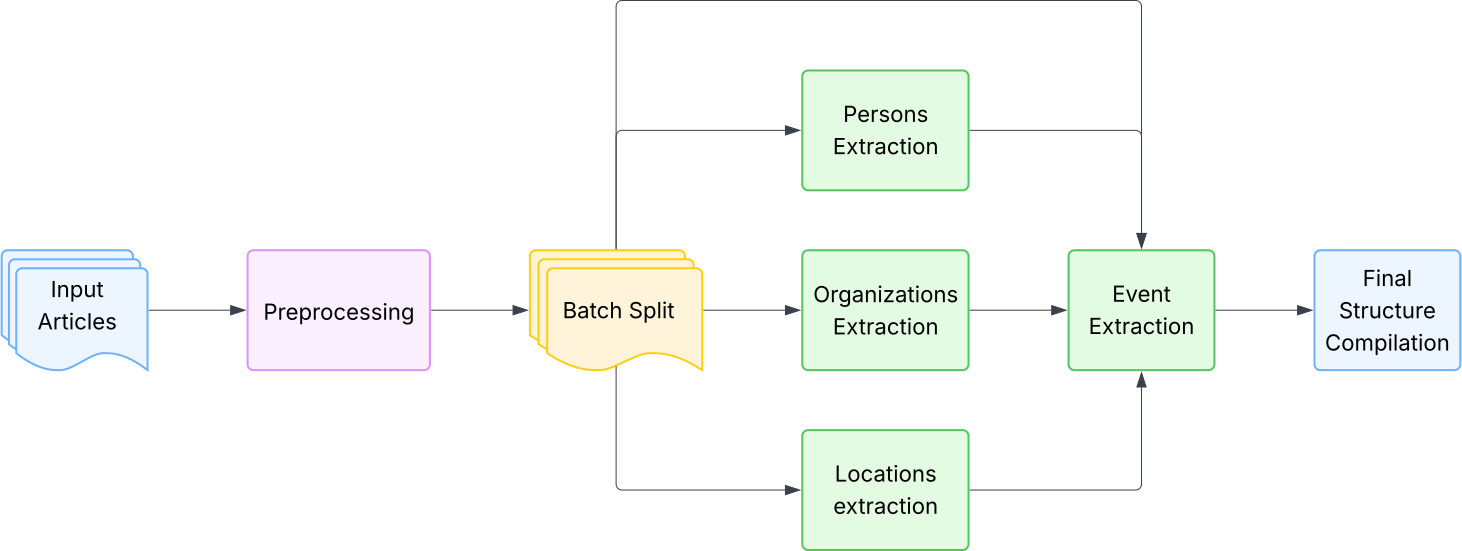
\includegraphics[height=0.65\paperheight]{figures/extraction-pipeline.png}
    \end{figure}
\end{frame}
%------------------------------------------------

%------------------------------------------------
\begin{frame}{Evaluation Framework}
\begin{itemize}
    \item \textbf{Extracted structure} against \textbf{Ground-truth} structure
    \item Custom evaluation pipeline: \textbf{Precision}, \textbf{Recall}, \textbf{F1} for entities, events and their assignments
    \item Entity matching using edit distance
    \item Event matching using semantic similarity
\end{itemize}
\end{frame}
%------------------------------------------------

%------------------------------------------------
\begin{frame}{Evaluation Dataset}
    \begin{itemize}
        \item Created ground-truth dataset
        \item 6 distinct media cases from different sections 
        \item Each case consists of 5 articles
        \item Total of 348 entities and 406 events
        \item Split: 1 case evaluation / 5 cases testing
    \end{itemize}
    \vspace{1em}
    \begin{columns}
        \begin{column}{0.45\textwidth}
            \colheader{Selected media cases}
            \begin{enumerate}
                \item Český lev Film Award
                \item Senate Elections 2018
                \item Olympic Games Beijing 2022
            \end{enumerate}
        \end{column}
        \begin{column}{0.45\textwidth}
            \begin{enumerate}
                \setcounter{enumi}{3}
                \item COVID-19
                \item Trump-Kim Summit
                \item Global Warming
            \end{enumerate}
        \end{column}
    \end{columns}
\end{frame}
%------------------------------------------------

%------------------------------------------------
\begin{frame}{Experimental Design}
\begin{itemize}
    \item Three pipeline versions:
    \begin{itemize}
        \item \textbf{V1}: Baseline, max batch
        \item \textbf{V2}: Prompt improvements
        \item \textbf{V3}: Single-article batch
    \end{itemize}

    \item Tested models:
    \begin{itemize}
        \item \textbf{Open-source} (Llama 4 Scout, Qwen3, DeepSeek R1)
        \item \textbf{Commercial} (Gemini 2.5 Pro, Gemini 2.5 Flash, GPT-4.1)
    \end{itemize}

\end{itemize}
\end{frame}
%------------------------------------------------

%------------------------------------------------
\begin{frame}{Results \& Discussion}
\begin{itemize}
    \item Solid results for baseline pipeline (0.57 F1 Score)
    \item Prompt engineering and batch size tuning provide marginal improvements
    \item Commercial LLMs outperform open-source
\end{itemize}

\begin{figure}
    \includegraphics[height=0.5\paperheight]{figures/pipeline-v1-precision-recall-bar-no-bg.pdf}
\end{figure}
    
\end{frame}
%------------------------------------------------

%------------------------------------------------
\begin{frame}{Conclusion}
% \textbf{Conclusion}:
\begin{itemize}
    \item Introduced a \textit{reproducible}, \textit{extendable} and \textit{modular} \textbf{extraction pipeline} for multi-document structured summarization

    \item Creation of the \textbf{validation dataset}

    \item Introduction of custom \textbf{evaluation framework} for structured data

    \item Thorough \textbf{analysis} of the proposed solution

    \item Demonstrated feasibility and highlighted trade-offs between model types

    \item Established a baseline for further methodological innovation
\end{itemize}

% \textbf{Future Directions}:

% \begin{itemize}
%     \item Improve deduplication and coreference across larger document sets

%     \item Experiment with automated prompt tuning and reasoning models

%     \item Extend to additional domains/languages
% \end{itemize}
\end{frame}
%------------------------------------------------

% Final PAGE
% Set the text that is showed on the final slide
\finalpagetext{Thank you for your attention}
%----------------------------------------------------------------------------------------
\makefinalpage
%----------------------------------------------------------------------------------------

\backupbegin

%------------------------------------------------
\begin{frame}{Opponent Questions}
\begin{block}{Question \#1}
    The results indicate that prompt and batch size optimization led only to marginal improvements. What fundamental changes might be required to overcome the current performance ceiling?
\end{block}

\begin{itemize}
    \item New prompt techniques (e.g. automatic prompt optimization)
    \item Fine-tuning the models for individual tasks
    \item Experiment with decoupled entity and event deduplication
    \item Revise the evaluation framework
\end{itemize}

\end{frame}
%------------------------------------------------

%------------------------------------------------
\begin{frame}{Opponent Questions}
\begin{block}{Question \#2}
    How would your framework handle a more structured extension beyond atomic events?
\end{block}

\begin{itemize}
    \item Matter of changing prompts and expected output schema
    \item Possible hierarchical tree structure of the events
    \item Evaluation either by evaluating sub-trees or by LLM-as-a-judge over the final tree structure
    \item Approach is currently being validated in our research group
\end{itemize}

\end{frame}
%------------------------------------------------

\begin{frame}{V1 Results}
    \centering
    \includegraphics[height=0.65\paperheight]{figures/suppport/pipeline-v1-precision-recall-bar.pdf}
\end{frame}

\begin{frame}{V1 Metrics comparison}
    \centering
    \includegraphics[height=0.65\paperheight]{figures/suppport/pipeline-v1-coord-per-metric.pdf}
\end{frame}

\begin{frame}{V1 Dataset comparison}
    \centering
    \includegraphics[height=0.65\paperheight]{figures/suppport/pipeline-v1-coord-per-dataset.pdf}
\end{frame}

\begin{frame}{V1 Stage comparison}
    \centering
    \includegraphics[height=0.65\paperheight]{figures/suppport/pipeline-v1-coord-per-stage.pdf}
\end{frame}

\begin{frame}{V2 Prompt tuning}
    \centering
    \includegraphics[height=0.65\paperheight]{figures/suppport/v1-iter-all.pdf}
\end{frame}

\begin{frame}{V2 Results}
    \centering
    \includegraphics[height=0.65\paperheight]{figures/suppport/pipeline-v2-precision-recall-bar.pdf}
\end{frame}

\begin{frame}{V3 Results}
    \centering
    \includegraphics[height=0.65\paperheight]{figures/suppport/pipeline-v3-precision-recall-bar.pdf}
\end{frame}

\begin{frame}{V1 - V2 Comparison}
    \centering
    \includegraphics[height=0.65\paperheight]{figures/suppport/v1-v2-f-diff.pdf}
\end{frame}

\begin{frame}{V1 - V2 Comparison}
    \centering
    \includegraphics[height=0.65\paperheight]{figures/suppport/v1-v2-data-points.pdf}
\end{frame}

\begin{frame}{V2 - V3 Comparison}
    \centering
    \includegraphics[height=0.65\paperheight]{figures/suppport/v2-v3-f-diff.pdf}
\end{frame}

\begin{frame}{V3 - V4 Comparison}
    \centering
    \includegraphics[height=0.65\paperheight]{figures/suppport/v2-v3-data-points.pdf}
\end{frame}

\begin{frame}{Temperature Influence}
    \centering
    \includegraphics[height=0.65\paperheight]{figures/suppport/temperature.pdf}
\end{frame}

\begin{frame}{Overall Performance}
    \centering
    \includegraphics[height=0.65\paperheight]{figures/suppport/model-performance-heatmaps.png}
\end{frame}

\backupend

\end{document}